% 
% Example SDSU Mathematics LaTeX Thesis.
% Lines beginning with % are comments and are ignored.
% 
% The class file sdsu-thesis.cls must be in the current directory or
% installed with the other classes as per standard LaTeX installation.
% 
% To generate run these commands:
% latex  thesis
% bibtex thesis
% latex  thesis
% latex  thesis
% Then you need to use the dvips command to get postscript output
% 
% See the README file for more information
% % tester
\documentclass{sdsu-thesis}
%
% 
% For early printouts to save paper use the savepaper option as
% 
% \documentclass[savepaper]{sdsu-thesis}
% 
% 
% This will make things single spaced, use small font and smaller
% margins.  Stuff will be formatted differently if you don't use this
% option but it's useful to basically see (read) what you typed so far
% on paper without wasting much paper.  You might want to also comment
% out the front matter and backmatter if printing out in savepaper
% mode to save paper there.  Do not use this option on your final
% printout as it doesn't satisfy the thesis manual requirements.

% Also if you want to use double spacing rather then singlespacing (if
% your thesis is very short, say 25 pages or less), then use he
% `doublespace' option as
% 
% \documentclass[doublespace]{sdsu-thesis}

% For including graphics use
% (Info) http://en.wikibooks.org/wiki/LaTeX/Importing_Graphics
%
% NOTE: My *may* need the graphicx package to get the correct
% page-size (letter) for your document... Some environments,
% e.g. TeXnicCenter default to 'a4' page size.
\usepackage{epsfig}
\usepackage{graphicx}

% These packages may also be useful for pictures...
% \usepackage{color}
% \usepackage{eepic}
% \usepackage{epic}
% \usepackage{grapic}


% Since this is a math thesis, you quite likely want these:
\usepackage{bm}
\usepackage{amsfonts}
\usepackage{amssymb}
\usepackage{amsthm}

% This makes captions *bold*
%
%(NOTE): Adding "justification=justified,singlelinecheck=false" to the
%        list of options will force all captions (including "short
%        one-line") to be left justified.  This is technically
%        required by the DTM, but looks ugly.
\usepackage[bf,labelsep=period,textfont=bf]{caption}

% Other useful packages for theses (see LaTeX docs for descriptions of these)
% 
% For the \vref commands that also prints out the reference page
% \usepackage{varioref}
% 
% For including computer code
% \usepackage{alltt}
% 
\usepackage{algorithm}
\usepackage{algpseudocode}

% For the \url{http://foo.com} command to include url's (or filenames)
% \usepackage{url}
% 
% For multi page tables
\usepackage{longtable}
%
% For correct "List of Tables" entry:
% (1) find the file "longtable.sty"
% (2) find the line
%     "\addcontentsline{lot}{table}{\protect\numberline{\thetable}{#2}}}%"
% (3) change to
%     "\addcontentsline{lot}{table}{\protect\numberline{Table\nobreakspace \thetable}{#2}}}%"


% This package countains the \sout command (which you should never use!)
\usepackage[normalem]{ulem}

%(GLOSSARY) (see %(GLOSSARY) below)
%(EXPERIMENTAL) --- Remove / Comment out if you don't need a glossary
\usepackage{datatool}
\usepackage[nonumberlist,section=paragraph]{glossaries}
\makeglossaries
\newacronym{lvm}{LVM}{Logical Volume Manager}

\newacronym{svd}{SVD}{Singular Value Decomposition}

\newglossaryentry{array}{
  name=array,
  description={A list of values identified by a numeric value}}

\newglossaryentry{binary}{
  name=binary,
  description={Pertaining to numbers represented in base 2}}

\newglossaryentry{comment}{
  name=comment,
  description={A remark that doesn't affect the meaning of the code}}

\newglossaryentry{global}{ 
  name=global,
  description={Something that maintains its state when it leaves the
    current group}}

\newglossaryentry{local}{
  name=local,
  description={Something that only maintains its state until it leaves
    the group in which it was defined/changed}} 

\newglossaryentry{quote}{
  name={"},
  description={the double quote symbol}}

\newglossaryentry{at}{
  name={@},
  description={the ``at'' symbol}}

\newglossaryentry{excl}{
  name={!},
  description={the exclamation mark symbol}}

\newglossaryentry{bar}{
  name={\ensuremath{|}},
  description={the vertical bar symbol}}

\newglossaryentry{hash}{
  name={\#},
  description={the hash symbol}}

\newglossaryentry{reals}{
  name={\ensuremath{\mathbb{R}}},
  description={the real numbers}}

\newglossaryentry{integers}{
  name={\ensuremath{\mathbb{Z}}},
  description={the integers}}

\newglossaryentry{rationals}{
  name={\ensuremath{\mathbb{Q}}},
  description={the rational numbers}}


\newtheoremstyle{dtm}% name of the style to be used
  {0pt}% measure of space to leave above the theorem. E.g.: 3pt
  {0pt}% measure of space to leave below the theorem. E.g.: 3pt
  {\slshape}% name of font to use in the body of the theorem
  {0pt}% measure of space to indent
  {\bfseries}% name of head font
  {. }% punctuation between head and body
  {0pt}% space after theorem head
  {}% Manually specify head
\theoremstyle{dtm}

% The style of theorems and such that you want to use.  You can change
% the style by modifying the second argument (for example prepending a
% formatting command, e.g. \textsc{Theorem} which will make the
% headings come out as small caps rather then bold).
% 
% On second thought, don't change these formats as you are likely to
% incur the wrath of the Thesis Reviewer.
% 
\newtheorem{corollary}{Corollary}[chapter]
\newtheorem{definition}{Definition}[chapter]
\newtheorem{lemma}{Lemma}[chapter]
%\newtheorem{proof}{Proof}[chapter]
\newtheorem{proposition}{Proposition}[chapter]
\newtheorem{theorem}{Theorem}[chapter]


% Author name and the author name in upper case
% (FORMAT) Has to match university records, check if you have
% (FORMAT) full middle name, or middle initital on record.
\author{Lloyd David Strohl III}

% Title of the thesis (all in upper case), use \\ for line breaks as
% usual, you can use up to 4 lines and make sure to set the counter
% titlelines to the number of lines you used.
% 
% This is for the title page
% 
\title{AN EVALUATION OF APOLLO \\
  POWERED DESCENT GUIDANCE }
% Number of lines in the title, without setting this the title page
% will not be formatted properly
\setcounter{titlelines}{2}

% Heading style title, the number of lines can be different here then
% in titlelines and in fact the thesis manual requires that this be at
% most 3 lines long so only put at most 2 pagebreaks here.  This is
% for the abstract pages and the signature page.
% 
% (FORMAT) Make sure that this title has the EXACT same words at the
% (FORMAT) title-page-title
% 
\titleheading{An Evaluation of Apollo \\
  Powered Descent Guidance}

%
% (FORMAT) The "degree" is set on three lines; select one of the
% following formats.  See DTM P.41
%
% Degree (MA-Math)
%\degreeONE{Master of Arts}
%\degreeTWO{in}
%\degreeTHREE{Mathematics}

% Degree (MS-Math)
%\degreeONE{Master of Science}
%\degreeTWO{in}
%\degreeTHREE{Mathematics}

% Degree (with Concentration)
\degreeONE{Master of Science in Aerospace Engineering}
\degreeTWO{with a Concentration in}
\degreeTHREE{Guidance, Navigation, and Controls}

% Degree (dual, concurrent)
%\degreeONE{Master of Science in Applied Mathematics}
%\degreeTWO{and}
%\degreeTHREE{Master of Science in Theoretical Typography}


% If you need to change the word 'Thesis' use \thesisname{Blah} and if
% you need to change the middle line between \degree and \degreein on
% the titlepage to something other then 'in' use \inofand{of} to use
% 'of' for instance.  (This should not be necessary)

% Dates
\gradyear{2018}
% (Format) Term Year 
\submitdate{Spring 2018}

% Your committee chair (don't include titles as per the manual)
\committeechair{Ping Lu}
\committeechairdept{Department of Aerospace Engineering}

% Second committee member
\committeesecond{Ahmad Bani Younes}
\committeeseconddept{Department of Aerospace Engineering}

% Third (usually different department) committee member
\committeethird{Peiman Naseradinmousavi}
\committeethirddept{Department of Mechanical Engineering}

%% Fourth is optional
%\committeefourth{Some Other Person}
%\committeefourthdept{Department of Otherness}


\begin{document}

% Title page 
% (FORMAT) Mandatory for SDSU thesis
\maketitle

% Signature page
% (FORMAT) Mandatory for SDSU thesis
\makesignature

% Copyright page
% (FORMAT) Mandatory for SDSU thesis
\begin{copyrightpage}
  Copyright~\copyright~2018 \\
  by \\
  Lloyd David Strohl III
\end{copyrightpage}

%% Dedication (make sure to format this correctly including a vspace
%% (say \vspace{3in} or using vfill) to make it center on the page if
%% desired, see the thesis manual) Or just delete this if you don't
%% have a dedication
%% 
%% (FORMAT) Optional
%\begin{dedication}
%  \vspace{3in}
%  \centering
%  Dedicated to me, as no one else is deserving.
%\end{dedication}

%% Epigraph (make sure to format this correctly, it will just be
%% centered on the page, see the manual) Or just delete this if you
%% don't have an epigraph
%% 
%% (FORMAT) Optional
%\begin{epigraph}
%  We must know, we shall know.\\
%  \begin{flushright}
%    -- David Hilbert
%  \end{flushright}
%\end{epigraph}

% Here type the abstract of your thesis.
% (FORMAT) Mandatory for SDSU thesis
\begin{abstract}
  % This just inserts the the abstract.tex file
  % You insert your abstract in the space below.


%This document is a summary of some relevant commands needed to create
%a Master's thesis for the Department of Mathematics and Statistics
%using \LaTeX. Included are examples of equations, figures, tables, and
%theorems. The formats listed in this document have been approved by
%the Department of Mathematical Sciences and the Graduate Division and
%Research.  If you have any difficulties with any of the driver or
%style files, please see your graduate adviser.

This is my abstract which describes my whole thesis. 

Many extraterrestrial missions require a powered descent phase. Because this phase is late in the mission its fuel efficiency has an outsized effect on payload capacity. This thesis presents a strategy for optimizing fuel use using well tested guidance algorithms that reduces fuel consumption over conventional strategies by x\%. 

\end{abstract}

% Table of contents
% (FORMAT) Mandatory for SDSU thesis
\tableofcontents

% If you don't want a list of tables page, delete or comment out this
% line
% (FORMAT) ONLY delete this page if you have *no* tables
\listoftables

% If you don't want a list of figures page, delete or comment out this
% line
% (FORMAT) ONLY delete this page if you have *no* figures
\listoffigures

%(GLOSSARY) (see %(GLOSSARY) above)
%(EXPERIMENTAL) --- Remove / Comment out if you don't need a glossary
% Glossaries
%\renewcommand*{\glsclearpage}{}
\begin{glossarypage}
%  \centering
  \glsaddall\printglossary[title=]
\end{glossarypage}


% Your acknowledgments go here
% Or just delete this if you don't have acknowledgments
% (you should! - Suck up to your advisor and committee!!!)
\begin{acknowledgments}
I would like to thank Dr. Lu for his serendipitous arrival at SDSU and consequent 
advice and instruction. With his mentoring I have been able to launch an enjoyable 
and fulfilling career in GN\&C, something I could not have achieved otherwise. 

%  I would like to thank Dr.~Gauss for allowing me to work on this
%  thesis even though he has been dead for so many years.  I would also
%  like to thank Dr.~Bolzano for not having any comments on this thesis,
%  and I would like to thank Dr.~Knuth for being the only living person
%  on my thesis committee, and for writing the wonderful \TeX.
%
%  This thesis is partially protected against the evil forces of the
%  Montezuma Publishing thesis reviewers by the magic of the Department
%  of Mathematics and Statistics Master's Thesis \LaTeX{} Template.
\end{acknowledgments}

%
% This is a diagnostic section to output the current font-selection is
% should be commented out... unless you're debugging font-selection,
% that is...
%
% Font parameters:
% \makeatletter
% \f@encoding -
% \f@family -
% \f@series -
% \f@shape -
% \f@size -
% \f@baselineskip -
% \tf@size -
% \sf@size -
% \ssf@size
% \makeatother


% 
% This includes body.tex
% 
% Note that if you want something in single space you can go back and
% forth between single space and normal space by the use of \ssp and
% \nsp.  If you want doublespacing you can use \dsp.  \nsp is normally
% 1.5 spacing unless you use the doublespace option (or savepaper
% option)
%
%(FORMAT) Usually you *don't* want to mess with the spacing for your
%(FORMAT) final version.  If you think/know that the thesis template
%(FORMAT) and/or thesis style file is incorrect/incomplete, PLEASE
%(FORMAT) contact the maintainer.  THANK YOU!!!

\chapter{INTRODUCTION}
\label{chap:intro}
% By labeling the chapter, I can refer to it later using the
% label. (\ref{chap:intro}, \pageref{chap:intro}) Latex will take care
% of the numbering.

You can save yourself 12 minutes now by not reading this document;
later on the average payback is 105-fold when you run into problems.

\section{History}

In the early 1990s Richard Frost put together a \LaTeX style file for
SDSU theses based on \LaTeX~2.09.  Joe Mahaffy wrote an example thesis
to guide students in the use of \LaTeX\ code.  Since that time \LaTeX
has been upgraded to \LaTeX2$\epsilon$ and the formatting requirements
for SDSU have also changed.  In 2004, Jiri Lebl and Mike O'Sullivan
worked on a revision, upgrading to \LaTeX2$\epsilon$.  This
\LaTeX2$\epsilon$ class file basically has almost nothing in common
with the old \LaTeX\ style; it is a modification of the standard
report class.

The class file \verb+sdsu-thesis.cls+ and this example are/have been
maintained by
\begin{itemize}
\item Aug 2010 --- \emph{current}: Peter Blomgren,
  \verb+<blomgren.peter@gmail.com>+.
\end{itemize}

In September 2010, the ``short'' example was merged into the ``long''
example to form this document; this seemed like a reasonable thing to
do.

While every effort is/has been made to make sure that the template and
thesis style conforms to the \emph{SDSU Thesis Manual}, \textbf{no
guarantees can be made.}  Depending on the thesis reviewer and his/her
interpreation of what is Really Important$^{\hbox{\scriptsize TM}}$ in
the thesis manual, and his/her level of caffeination some theses fly
through, and some get stuck even though they use the same template and
style file.

PLEASE let the maintainer know of any and all feedback you get from
the thesis reviewer so that the template and/or style file can be
updated as necessary.  THANK YOU!!!


\section{Purpose}

This document illustrates some of the typesetting tasks that are
commonly encountered in a thesis containing
mathematics\footnote{\texttt{http://en.wikibooks.org/wiki/LaTeX}\quad
  provides a wealth of information regarding \LaTeX, check it out.}.
All theses must follow the guidelines of the SDSU Thesis Manual for
formating.  Most formating issues will be automatically handled by the
\LaTeX\ class file included with the source file for this document,
but there may be some special circumstances that will require some
tinkering with spacing, pagebreaks, etc.

\LaTeX\ is a remarkably powerful package, but it does take some effort
to learn.  The best plan is to start with something already written
and learn from the example.  The current document was produced for
this purpose.  This document illustrates how the student should format
the chapters and sections of the thesis, prepare the bibliography, and
include other appropriate items commonly found in a technical
document.  The title page, signature page, acknowledgments page,
abstract, and everything else are all formatted according to
specifications of the SDSU Thesis Manual of 2004, once you enter the
text to include.

For a general reference it is recommended that the student obtain the
user's guide and reference manual of Leslie Lamport \cite{LAM}. The
student should obtain copies of the files used to generate this
document, then examine the ASCII files used to generate the document
and the \LaTeX\ output.  The files for this example thesis are the
following.
\begin{itemize}
\item \verb+Makefile+: Contains ``recipes'' for building the thesis;
  type typing \verb+make+, and \verb+make thesis.pdf+.
\item \verb+abstract.tex+: Contains the abstract.
\item \verb+append.tex+: Contains all the text for appendices.
\item \verb+body.tex+: Contains all the text for chapters. 
\item \verb+sdsu-thesis.cls+: Defines the layout and formatting.
\item \verb+thbib.bib+:  Contains a bibliographical database.
\item \verb+thesis.tex+: 
  \begin{enumerate}
  \item  Contains information for the title page, and other
    front-matter.
  \item Includes the files \verb+abstract.tex+,  \verb+body.tex+, and
    \verb+append.tex+. 
  \item Defines the bibliographical style (\verb+siam+ in this
    example) and creates the bibliography using the file
    \verb+thbib.tex+.
  \end{enumerate}
\item \verb+cos.eps+, \verb+mapping.eps+, \verb+plot2.eps+, and
  \verb+somb.eps+: Encapsulated postscript files that are included by
  \verb+body.tex+ (in the subdirectory \verb+Figures/+.)
\end{itemize}

Positioning and captioning of figures and tables should agree with the
thesis manual.  Occasionally, \LaTeX\ does not break when you want it
too, so you have to add a \verb+\newpage+ command to get
the correct break, such as when a section header starts at the bottom
of a page or when paragraphs have widows or orphans.


\section{Format of the Thesis}
The Department of Mathematics and Statistics wants the student to use
a standard technical format. This implies that equations, theorems,
definitions, tables, etc. should be numbered $N.M$, where $N$ is the
chapter number and $M$ is successively increased through the chapter.
\LaTeX\ does this automatically. Numbering of the equations is on the
right side of the page (default in \LaTeX).  The student may use
\textit{italics}, \textsc{small caps}, or \textbf{bold fonts} to
highlight important phrases.  The code for creating theorems,
definitions etc., is illustrated in this example thesis.  Positioning
and captioning of figures and tables should agree with the thesis
manual.  Occasionally, \LaTeX\ does not break when you want it too, so
you have to add a \verb+\newpage+ command to get the correct break,
such as when a section header starts at the bottom of a page or when
paragraphs have widows or orphans.

Bibliographical citations are relatively easy.  Here is one \cite{ART}
and another citation \cite{Lehto:1976} and we can't forget Milnor
\cite{Milnor:topdiff}.  Look at \verb+thbib.bib+ to see how to create
the database for the bibliography.

You type new paragraphs by just leaving an empty line between them.



\section{Processing \LaTeX\ Files}

The best way to learn \LaTeX\ is to take advantage of someone else's
work from which you can model your document. This pseudo-thesis should
give you a good working example to create your own document. The key
commands to create any document are the following: \vspace{.15in}

\noindent\texttt{%
  \ssp % \ssp inside the { } makes the change temporary
  \hspace*{5em}$\backslash$documentclass[\emph{options}]\{\emph{class}\}\\
  \hspace*{5em}$\backslash$begin\{document\}\\
  \hspace*{7em}Insert any text you want in here.\\
  \hspace*{5em}$\backslash$end\{document\}\\
}

\noindent
where \emph{class} is some class type.  For SDSU Thesis you would
normally use the \texttt{sdsu-thesis} class.  When you're writing your
thesis and want a draft printout you can also add options such as
\texttt{savepaper} which will single space your document, and use
larger margins.  Most postscript viewers will allow you to print only
a subset of pages as well.  The standard for the final thesis is $1
\,1/2$ space.  If you want double spaced then uncomment the
\texttt{doublespace} option.

\verb+README+ files for the different operating systems accompany this
distribution.  Here we explain how to use the command line to process
\LaTeX\ on a Unix/Linux system (or with modifications Mac OS X).

To process a \LaTeX\ document that you have named
\texttt{filename.tex}, you simply type \texttt{latex filename}. For
example, this document is generated by its driver file with
\texttt{latex thesis}. If it is the first time and you have a
bibliography, then you need the following sequence of commands:
\vspace{.15in}

\noindent\texttt{%
  \ssp % \ssp inside the { } makes the change temporary
  \hspace*{5em}latex filename\\  
  \hspace*{5em}bibtex filename\\
  \hspace*{5em}latex filename\\
  \hspace*{5em}latex filename\\
}
\vspace{.15in}

\noindent
Unless you have added new references, the \texttt{bibtex filename} can
be omitted. You will need to execute the \texttt{latex filename}
command twice if there are any renumbering of items, like
equations. When there are errors you can usually hit the carriage
return and work through them\footnote{Do not panic if you get lots of
  errors; fix the \emph{first} one!  The following errors are often
  due to things being out-of-context due to the first error. ALWAYS
  fix the first error before worrying about the others!!!  \emph{ALWAYS
    fix the first error before worrying about the others!!!}
  \textbf{ALWAYS fix the first error before worrying about the
    others!!!}}.  Other alternatives include typing either \texttt{x}
or \texttt{q} to allow it to proceed. The errors will be kept in a
file called \texttt{filename.log}.  Be sure to pay attention to
comments the \LaTeX\ produces as it gives you some warnings, such as
when you need to make another run due to changes in the numbering of
references or equations.

After you have performed the above procedure, you will have a file
named \texttt{filename.dvi} (or \texttt{thesis.dvi} in our case) which
is a device independent file. There are several means of viewing your
output. If you are working in an Xwindow environment, then the
simplest procedure is to type \texttt{xdvi filename.dvi}, which will
open a window for viewing the \LaTeX\ document. It will not include
any postscript figures, but it is automatically updated each time you
latex your document. I highly recommend starting with this
environment. (If you are on rohan and accessing saturn, then you will
need the environment setup described below for ghostview.)

The second procedure for either viewing with ghostview or printing
involves the conversion of the .dvi file to a postscript file. (You
may want to examine \texttt{man dvips} for assistance.) The simplest
way to convert the .dvi file to a postscript file is to type the
following: \vspace{.15in}

\texttt{
  dvips -o filename.ps filename.dvi
}
\vspace{.15in}

\noindent
This creates the postscript file, \texttt{filename.ps}. If you do not
need the entire document, then you can type: \vspace{.15in}

\texttt{
  dvips -p\emph{x} -l\emph{y} -o filename.ps filename.dvi
}
\vspace{.15in}

\noindent
where \texttt{x} is the number of the first page and \texttt{y} is the
number of the last page.

Then to get a hard copy you should use the standard printing commands
of your system.  If you are on your own Linux system at home, usually
\texttt{lpr filename.ps} will print the file.

In case your computer system has a different paper size set up as
default then ``letter'' you can force a letter paper size by adding
\texttt{-t letter} as an option to \texttt{dvips}.  This can happen if
you are running in a different language then American English.

The makefile simplifies many of the sequences of commands that you
might use.  For example, just type \texttt{make} to create a
postscript file or \texttt{make view} to create a postscript and view
it using a postscript viewer. Also, make clean will remove all the
.log .aux .ps .dvi files.




\chapter{MISCELLANEOUS COMMANDS: AN INTRODUCTION TO EQUATIONS,
  THEOREMS, FIGURES AND TABLES}

In this chapter we see how equations, theorems, figures and tables are
created, enumerated and referenced.  We also play around with lengths
of chapter and section headings.  For example, this chapter begins
with a long chapter heading that must conform to the thesis manual.
Later on there is a very long section heading.  These examples show
how the sdsu thesis class file automatically handles formating.



\section{Basic Math}

You can have fun formulas, such as $x= 7 y^x$.  If you want the
equations displayed you can use two dollar signs, \$\$ to enclose the
mathematics, or you can use

\medskip\noindent
\texttt{%
  \hspace*{2em}$\backslash$begin\{equation*\} \\
  \hspace*{3em}math stuff \\
  \hspace*{2em}$\backslash$end\{equation*\}
}\\%
as in

\medskip\noindent\hspace*{2em}\begin{minipage}{4.5in}
\begin{verbatim}
\begin{equation*}
  \int_{\partial \Omega} \omega = \int_{\Omega} d\omega.
\end{equation*}
\end{verbatim}
\end{minipage}

\medskip\noindent
which produces
\begin{equation*}
  \int_{\partial \Omega} \omega = \int_{\Omega} d\omega.
\end{equation*}

There are several other ways to display equations.  The code for this
one (which you can see in \verb+body.tex+) aligns all the equal
signs.
\begin{align}
  (x+2)^3 & = (x+2)(x+2)^2 \\
  &= (x+2)(x^2+4x+ 4) \\
  &= x^3+ 6x^2 + 12*x + 8
\end{align}
Notice that this last set of equations is numbered, but the previous
one is not.  The * in the \LaTeX\ code eliminates the numbering.


\section{Equations}

Enumeration of equations, theorems, definitions, tables, is handled
automatically by \LaTeX.  Each of these items may be given a label
using \verb+\label{<labelname>}+.  The item can then be refered to
by \verb+\ref{<labelname>}+.  Below we demonstrate how
to create and label an equation. Our first is a general differential
equation,
\begin{equation}
  \dot{x} = f(t,x),\qquad x(0)= x_0. \label{de1}
\end{equation}
To see that the numbering is going fine we insert a matrix system as
follows:
\begin{equation}
  \dot{y} =
  \begin{bmatrix}
    a_1 & 0 & \cdots & 0 \\
    0 & a_2 & \cdots & 0 \\
    \vdots & \vdots & \ddots & \vdots \\
    0 & 0 & \cdots & a_n
  \end{bmatrix}
  y.
  \label{de2}
\end{equation}
The numbering is valuable when one wants to refer to the
Equations~(\ref{de1}) and (\ref{de2}). Note that when referring to
Equation~(\ref{de1}) you must capitalize the word equation. Also, when
you enter a specific equation, figure, or table, \emph{e.g.,}
Eqn.~(\ref{de1}), then you should type a $\tilde{\phantom{x}}$ between
the word Eqn., Fig., or Table and its labeling number to prevent
inappropriate division of the label at the end of a line.

To display an equation without numbering, one uses the math
displaystyle mode which works as follows:
\begin{equation*}
  \dot{y} = g(y),
\end{equation*}
which is an autonomous equation in $y$. The $y$ at the end of the last
sentence is in standard math mode. Further information on equations is
provided in Appendix~A.


\section{Theorems, etc.}

The student needs to highlight important results such as theorems,
hypotheses, or definitions. In this section we investigate how
\LaTeX\ handles definitions, theorems, corollaries, etc.
\begin{definition}   
  A linear differential equation is asymptotically stable if and only
  if all eigenvalues, $\lambda$, of the operator matrix have negative
  real part.
\end{definition}
We follow this with a couple of theorems and a corollary.
\begin{theorem}
  If the matrix $A$ in the linear differential equation,
  \begin{equation}
    \dot{y} = Ay, \qquad y(0) = y_0, \label{lde}
  \end{equation}
  is symmetric, then the solution of {\rm (\ref{lde})} is
  non-oscillatory.
\end{theorem}
\begin{corollary}
  If the matrix $A$ in {\rm (\ref{lde})} is symmetric and has negative
  eigenvalues, then the solution is non-oscillatory and asymptotically
  stable.
\end{corollary}

In order to check how the numbering proceeds we insert here another
theorem.
\begin{theorem}
  If the matrix $H$ in the linear differential equation,
  \begin{equation}
    \dot{y} = Hy, \qquad y(0) = y_0, \label{ldeh}
  \end{equation}
  is antisymmetric, then the solution of {\rm (\ref{ldeh})} is oscillatory.
\end{theorem}

The \texttt{thesis.tex} also defines environments for \texttt{lemma}
and \texttt{proposition} though you can add more if you wish.  For
example sometimes it is useful to add an \texttt{example} style
environment.  See the preamble of the document for more information.
















\section{Optimal Powered Descent Guidance Law}
Derivation of an optimal powered descent guidance law begins with a formulation of the State Equation\phantom{x}\ref{eqn:state_equation}
\begin{equation}
\dot{\boldsymbol{x}} = \boldsymbol{f}(\boldsymbol{x})
\label{eqn:state_equation}
\end{equation}

The state equations for the 3-dimensional powered descent guidance problem are as follows

\begin{align}
\label{eqn:EoM1}
\boldsymbol{\dot{r}} &= \boldsymbol{V}                               & \boldsymbol{r(t_0)} &= \boldsymbol{r_0}\\
\label{eqn:EoM2}
\boldsymbol{\dot{V}} &= \boldsymbol{g(r)} + \boldsymbol{a_T}                           & \boldsymbol{V(t_0)} &= \boldsymbol{V_0}
\end{align}

%Where 
%\begin{align*}
%\dot{m} &= -\frac{T}{g_0 I_{sp}} & m(t_0) &= m_0\\
%a &= \frac{T}{m(t)} \\
%\end{align*}

with terminal constraints at a fixed final time $t_t$
\begin{align}
\label{eqn:constraint_r}
\boldsymbol{r}^*(t_f) &= \boldsymbol{r}^*_f\\
\label{eqn:constraint_V}
\boldsymbol{V}(t_f) &= \boldsymbol{V}^*_f 
\end{align}

where $\boldsymbol{a}_T$ is the thrust acceleration vector. $\boldsymbol{a}_T$ is limited such that
\begin{equation} 
\label{eqn:thrustlimit}
0 < a_{min} \leq ||\boldsymbol{a}_T|| \leq a_{max}
\end{equation}

\subsection{Performance Index}
Fuel consumption is related to the thrust acceleration vector by engine parameters represented by some positive constant k

\begin{equation}
\label{eqn:fuel_rate}
\dot{m} = -k ||\boldsymbol{a}_T||
\end{equation}

A fuel optimal guidance law should therefore use the performance index
\begin{equation}
\label{eqn:fueloptimalindex}
J = \int_{t_0}^{t_f} ||\boldsymbol{a}_T||dt
\end{equation}

Choosing to minimize the square of the total acceleration $\boldsymbol{a} = \boldsymbol{g} + \boldsymbol{a}_T$ gives a performance index
\begin{equation}
\label{eqn:performanceindex}
J = \frac{1}{2} \int_{t_0}^{t_f} (\boldsymbol{g}+\boldsymbol{a}_T)^T(\boldsymbol{g}+\boldsymbol{a}_T)dt
\end{equation}

For a constant gravitational acceleration $\boldsymbol{g}$, this performance index attempts to minimize $||\boldsymbol{a}_T||^2$. It is not fuel optimal as in Equation \ref{eqn:fueloptimalindex}, but it does provide a cost to large thrust accelerations and might be expected to give good fuel performance.

\subsection{Guidance solution}
Choosing the guidance command $\boldsymbol{u} = \boldsymbol{g} + \boldsymbol{a}_T$ and applying optimal control theory results in the following
\begin{equation}
\label{eqn:Hamiltonian}
H = \boldsymbol{p}_r^T\boldsymbol{V} + \boldsymbol{p}_V^T\boldsymbol{u} - \frac{1}{2}\boldsymbol{u}^T\boldsymbol{u}
\end{equation}

\begin{equation*}
\dot{\boldsymbol{p}}_r = -\frac{\partial H}{\partial \boldsymbol{r}} = 0 \implies \boldsymbol{p}_r = -\boldsymbol{c}_2
\end{equation*}
\begin{equation*}
\dot{\boldsymbol{p}}_V = -\frac{\partial H}{\partial \boldsymbol{V}} = -\boldsymbol{p}_r \implies \boldsymbol{p}_V = \boldsymbol{c}_1 + \boldsymbol{c}_2 t
\end{equation*}
\begin{equation*}
\frac{\partial H}{\partial \boldsymbol{u}} = 0 \implies \boldsymbol{u} = \boldsymbol{p}_V = \boldsymbol{c}_1 + \boldsymbol{c}_2 t
\end{equation*}

For convenience, let $\tau = t_f - t$
\begin{equation}
\label{eqn:command}
\boldsymbol{u} = \boldsymbol{k}_1 + \boldsymbol{k}_2 \tau
\end{equation}
where $\boldsymbol{k}_1$ and $\boldsymbol{k}_2$ are constant vectors.

Integrating the equations of motion with $\boldsymbol{\dot{V}} = \boldsymbol{u}$ then gives
\begin{equation}
\label{eqn:EoM_solve_1}
\int\boldsymbol{\dot{V}}(t) dt  = \boldsymbol{k}_1(t-t_0) + \frac{1}{2}\boldsymbol{k}_2(t-t_0)^2 + \boldsymbol{V}(t_0) 
\end{equation}

\begin{equation}
\int \boldsymbol{\dot{r}}(t)dt = \frac{1}{2} \boldsymbol{k}_1(t-t_0)^2 + \frac{1}{6}\boldsymbol{k}_2(t-t_0)^3 + \boldsymbol{V}(t_0)(t-t_0) + \boldsymbol{r}(t_0) 
\label{eqn:EoM_solve_2}
\end{equation}

Setting $t = t_f$ and letting $t_{go} = t_f - t_0$ satisfies the terminal constraints from Equations \ref{eqn:constraint_r} and \ref{eqn:constraint_V}, resulting in 6 linear equations in 6 unknowns

\begin{align}
\label{eqn:system1}
\boldsymbol{k}_1 t_{go} + \frac{1}{2}\boldsymbol{k}_2 t_{go}^2 &= \boldsymbol{V}_f^* - \boldsymbol{V}_0\\
\label{eqn:system2}
\frac{1}{2}\boldsymbol{k}_1 t_{go}^2 + \frac{1}{6}\boldsymbol{k}_2 t_{go}^3 &= \boldsymbol{r}_f^* - \boldsymbol{r}_0 - \boldsymbol{V}_0t_{go}
\end{align}

These equations can be separated into sets of two per vector component. Define an inertial guidance frame $\boldsymbol{e} = (\hat{x},\hat{y},\hat{z})^T$ such that guidance vector $\boldsymbol{u}$ is composed of components in $\boldsymbol{e}$, $\boldsymbol{u} = (u_{x},u_{y},u_{z})^T$. For the equations in $\hat{x}$ we have

\begin{equation}
  \begin{bmatrix}
    t_{go} & \frac{1}{2}t_{go}^2 \\
    \frac{1}{2}t_{go}^2 & \frac{1}{6}t_{go}^3 \\
  \end{bmatrix}
 \left(
	\begin{matrix}
	k_{1_x} \\ 
	k_{2_x} 
	\end{matrix}
\right) = 
 \left(
	\begin{matrix}
	V_{f_x}^* - V_{0_x} \\ 
	r_{f_x}^* - (r_{0_x} + V_{0_x}t_{go}) 
	\end{matrix}
\right)
%  \label{de2}
\end{equation}

Solving the two-equation system is accomplished by inverting the A matrix, leading to a coefficient matrix $E$
\begin{equation}
E = 
	\begin{bmatrix}
	-2/t_{go} & 6/t_{go}^2 \\
	6/t_{go}^2 & -12/t_{go}^3
	\end{bmatrix}
\end{equation}

The coefficients in $\hat{x}$ are then
\begin{equation}
\begin{pmatrix}
k_{1_x} \\
k_{2_x}
\end{pmatrix}
= E
\begin{pmatrix}
V_{f_x}^* - V_{0_x} \\ 
r_{f_x}^* - (r_{0_x} + V_{0_x}t_{go}) 
\end{pmatrix}
\end{equation}

It can be shown that the equations in $\hat{y}$ and $\hat{z}$ take the same form. This $2x2$ $E$ matrix is the origin of the name \textit{E-Guidance}, the guidance law used in the Apollo lunar landing missions.

\subsection{Time-to-go}
The E-Guidance solution depends upon a reliable estimate of remaining time-to-go ($t_{go}$). The Apollo mission's guidance used an estimate that updated continuously using Newton's method, but it was intended to only operate until start of the terminal descent phase at which point guidance switched to a manual vertical descent operation. Updating the $t_{go}$ estimate continuously is attractive since it should be robust; if conditions have to change during the mission a closed-loop (continuously updating) solution will adjust and a new, realistic $t_{go}$ will feed into the guidance solution. This quality was important to the Apollo Guidance solution because it relied upon pilot inputs to define the landing location visually, which meant allowing for landing site redesignations mid-mission. If $t_{go}$ was not recomputed after site redesignation, the guidance law would impose unrealizable thrust acceleration commands.

For the purposes of this study, live landing site redesignation was not considered. Without the possibility of landing site redesignation, an open-loop $t_{go}$ solution lends the guidance law more stability in that the performance is less dependent upon specific assumptions and conditions imposed by the $t_{go}$ algorithm. For instance, one closed-loop $t_{go}$ algorithm is implemented as follows

\begin{align}
while 
\label{eqn:tgoFPI}
\Delta V &= \sqrt{(\boldsymbol{V}-\boldsymbol{V_0} + \boldsymbol{g}\cdot t_{go})^T(\boldsymbol{V}-\boldsymbol{V_0} + \boldsymbol{g}\cdot t_{go})} \\ 
5 = g
\end{align}

\begin{algorithm}
\begin{algorithmic}
	\State $tol \gets 1$ 
	\If {$i\geq maxval$}
	\State $i\gets 0$
	\Else
	\If {$i+k\leq maxval$}
	\State $i\gets i+k$
	\EndIf
	\EndIf
\end{algorithmic}
\end{algorithm}


This algorithm requires an assumption about a fixed mass flow rate which is not guaranteed by the guidance law. Adjustment of this mass flow rate estimate is very particular to the initial conditions of the mission, resulting in a necessarily over conservative $t_{go}$ to account for initial condition dispersion.





\section{Figures or How to Get into Real Trouble if You Take Advantage
  of What \LaTeX\ Can Do}

This section shows how to display figures and refer to them in the
text.  \LaTeX\ does have the ability to insert postscript files using
the \verb+graphicx+ package.  Make sure to include
\verb+\usepackage{graphicx}+ in your preamble, that is between the
\LaTeX\ commands \verb+\documentclass+ and
\verb+\begin{document}+. \emph{See}
  \verb+http://en.wikibooks.org/wiki/LaTeX/Importing_Graphics+
  \emph{for information about importing graphics into your
    document.}

To insert a figure that is formatted in encapsulated postscript, which
must include a Bounding Box line which is named \texttt{fname.ps} you
do the following:
\\
\texttt{ \hspace*{0.5in} $\backslash$begin\{figure\}[ht]
  \\
  \hspace*{0.75in}
  $\backslash$includegraphics[width=$\backslash$linewidth]\{fname.eps\}
  \\
  \hspace*{0.75in} $\backslash$caption\{Insert a caption
  here. $\backslash$label\{figlabel\} \}
  \\
  \hspace*{0.5in} $\backslash$end\{figure\} }
\\
to produce the figure. The \textbf{[ht]} argument to the figure
command is a \emph{suggestion} to \LaTeX\ to put the figure
\textbf{[h]}ere, or at the \textbf{[t]}op of the page; \textbf{[p]}
for a separate page is also possible.
Avoid\marginpar{\small\textbf{\textit{Style note}}} putting tables and
figures at the \textbf{[b]}ottom of the page as this is frowned upon
by the thesis manual; the
preference\marginpar{\scriptsize\raggedright\textbf{NEVER put anything
    in the margin like this!!!}} is to put tables and figures right
after they are first referenced, \emph{i.e.}\ \textbf{[h]}ere, but
at the \textbf{[t]}op of the following page is acceptable in cases
where it does not fit \textbf{[h]}ere.  You can make the suggestion
stronger by saying \textbf{[h!]}  for ``\textbf{[h]}ere\textbf{!},''
but the internal rules may still override your suggestion.
``\verb+\linewidth+'' above can be replaced by some
number of inches (or other size \LaTeX{} size measure such as
\texttt{pt}, \texttt{em}, or \texttt{ex}).  This will left justify the
figure.  Centering is a little more complicated.  We place everything
in a \texttt{minipage} environment:
\\
\texttt{ \hspace*{0.5in} $\backslash$begin\{figure\}[ht]
  \\
  \hspace*{0.75in} $\backslash$centering
  \\
  \hspace*{0.75in} $\backslash$begin\{minipage\}\{$x$in\}
  \\
  \hspace*{1.0in}
  $\backslash$includegraphics[width=$\backslash$linewidth]\{fname.ps\}
  \\
  \hspace*{1.0in} $\backslash$caption\{Insert a caption
  here. $\backslash$label\{figlabel\} \}
  \\
  \hspace*{0.75in} $\backslash$end\{minipage\}
  \\
  \hspace*{0.5in} $\backslash$end\{figure\} }

To demonstrate how the department would like to see figures in the
thesis the following is provided. If you are examining these files
with \texttt{xdvi}, you will only see a blank spot. However, both
printed and ghostview methods described in the previous chapter will
allow viewing.  Suppose that we create a figure to graph the curve
\begin{equation}
  y=\sin(\omega t), \label{gr1}
\end{equation}
where $\omega$ is the circular frequency.  Figure~\ref{fig1} is a
graph of Equation~(\ref{gr1}), and figure~\ref{fig:graph} is an
illustration of a mapping in the complex plane. The interval of time
viewed is $t \in [-5,5]$. The figure reference should be denoted by
either Fig.~\ref{fig1} or by Figure~\ref{fig1} with specific figures
capitalized as noted here.
%\begin{figure}[ht]
%  \centering
%  \begin{minipage}{4.5in}
%    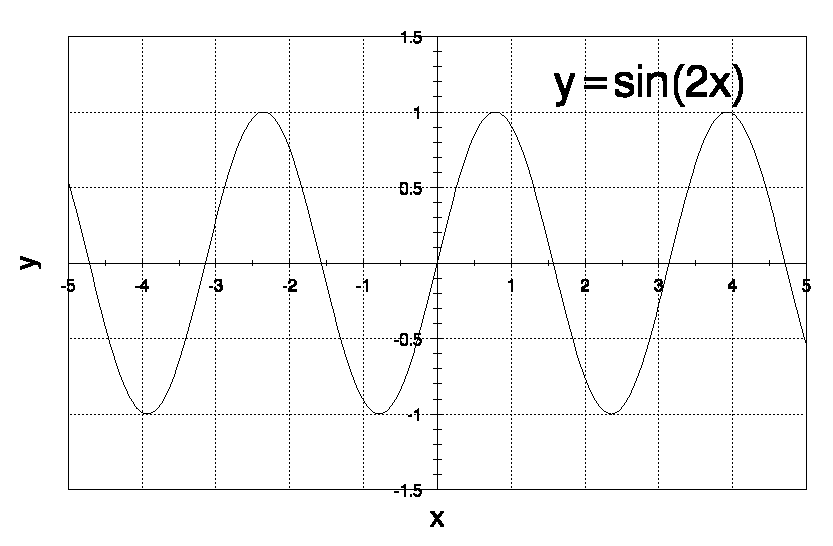
\includegraphics[width=\linewidth]{Figures/plot2.eps}
%    \caption{This is a graph of the above equation, where the circular
%      frequency is taken as $\omega = 2$.\label{fig1} Note: \emph{if
%        you need to cite a source (of e.g.~a figure) in the caption,
%        include the FULL CITATION, e.g.~} Source: Montezuma
%      Publishing, San Diego State University Dissertation and Thesis
%      Manual: Policies, Procedures and Format, Spring
%      2010. \cite[\S 4.10.4 Figures]{DTM2010spring}}
%  \end{minipage}
%\end{figure}

%\begin{figure}[ht]
%  \centering
%  \begin{minipage}{4.5in}
%    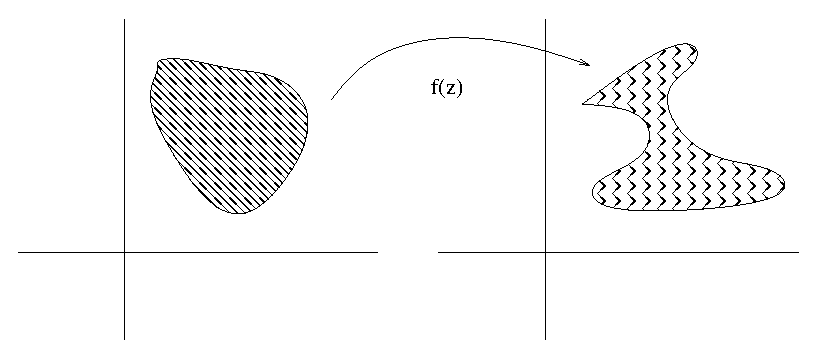
\includegraphics[width=\linewidth]{Figures/mapping.eps}
%    \caption{Mapping $f(x)$ from the complex plane to itself. \label{fig:graph}}
%  \end{minipage}
%\end{figure}


When you have a collection of figures and large figures, you may want
to delay insertion of them until the end of the chapter. At the end of
this chapter we are including a full page figure (Fig.~\ref{fullfig})
to demonstrate this \LaTeX\ command. Note that if you cannot obtain
postscript figures or are having too much trouble using the technique
described above, then you can use the \verb+\vspace+ command to
provide an empty space in the manuscript, then use the old-fashioned
technique of taping in your figure and photocopying it.

% 
% If you have oversize full page figures, the following
% might come in handy
% 
% \figurecoversheet{\label{figure:oversize} Caption goes here}


\section{Tables}

The Department of Mathematical Sciences does not have specific
requirements on the exact layout of a table. However, the tables
should be easily readable and properly labeled according to the
regulations in the SDSU Thesis Manual. In this section we want to
demonstrate how \LaTeX\ handles tables. More complicated examples can
be found in Lamport's book \cite{LAM,LAM2}. We begin with a small table,
given by Table \ref{tab1} which inserts nicely into the text.  Note
that the same centering trick as was employed for figures is done here
and we set the width of the \texttt{minipage} environment to 1.9
inches.
% 

\begin{table}[hbt]
  \centering
  \begin{minipage}{1.9in}
    \caption{A Small Table for Listing Some Parameters Used in Some
      Numerical Procedure\label{tab1}. LONG CAPTION--- The Department
      of Mathematical Sciences does not have specific requirements on
      the exact layout of a table. However, the tables should be
      easily readable and properly labeled according to the
      regulations in the SDSU Thesis Manual.}
    \begin{tabular}{|c||c|c|c|c||}    \hline
      Trial &	a  &  b & c & $\omega$ \\ \hline \hline
      1 & 5 & 10  & 15 & $\pi$ \\ \hline
      2 & 10 & 20  & 15 & $2\pi$ \\ \hline
    \end{tabular}
  \end{minipage}
\end{table}
% 

The\marginpar{\small\textbf{\textit{Style note}}} manual however
allows for the caption to be a little wider if the table is really
small and so we can use a wider \texttt{minipage} and then center the
table inside there.  See for example Table \ref{wtab} where we used
width of 3.5 inches.
% 
\begin{table}[hbt]
  \centering
  \begin{minipage}{3.5in}
    \centering
    \caption{Another Small Table for Listing Some Parameters Used in a
      Numerical Procedure\label{wtab}.}
    \begin{tabular}{|c||c|c|c|c||}    \hline
      Trial &	a  &  b & c & $\omega$ \\ \hline \hline
      1 & 5 & 10  & 15 & $\pi$ \\ \hline
      2 & 10 & 20  & 15 & $2\pi$ \\ \hline
    \end{tabular}
  \end{minipage}
\end{table}

Note that you can use the \texttt{center} environment instead of
\texttt{$\backslash$centering} but that might add a little bit of
unwanted whitespace.  With \texttt{$\backslash$centering} on the other
hand, you might have to put braces around the text you wish to center
and sometimes need to add a \texttt{$\backslash$par}.  If you use it
inside a \texttt{minipage}, \texttt{table} or \texttt{figure}
environment, you don't have to really worry about that.  Note however
that without the use of \texttt{minipage} you cannot center the
caption as it automatically left aligns itself to conform with the
thesis manual.

Tables can also be left aligned see for example Table \ref{ltab}.
Here we don't use the \texttt{minipage} environment, but we must then
add linebreaks so that the table caption does not go wider then the
table itself.  We need to add then two titles, one for the list of
tables and one for the caption here.  The former will not have line
breaks and the latter will.
% 
\begin{table}[hbt]
  \caption[
  Another Such Table but Left Aligned]{
    Another Such\\Table but Left Aligned\label{ltab}}
  \begin{tabular}{|c||c|c|c|c||}    \hline
    Trial &	a  &  b & c & $\omega$ \\ \hline \hline
    1 & 5 & 10  & 15 & $\pi$ \\ \hline
    2 & 10 & 20  & 15 & $2\pi$ \\ \hline
  \end{tabular}
\end{table}

Sometimes a table might not fit onto a single page, in this case you
must not use the \texttt{table} environment, but instead the
\texttt{longtable} environment.  Do note that \texttt{longtable}
automatically centers so you need not worry about that.  See Table
\ref{totallyrandom} for some absolutely random numbers.  To use
\texttt{longtable} environment you must include the \texttt{longtable}
package in your preamble. \textbf{see the note in \texttt{thesis.tex}
  on how to fix the longtable entries in the ``List of Tables'' if
  they are incorrect.}

\begin{longtable}{|l|l|l|}
  % You may need to modify the \LTcapwidth if the title wraps too early, or
  % if it makes your table too large
  % \LTcapwidth=6in
  \caption{A Table of Some Totally Random Numbers} \label{totallyrandom} \\

  % Here are our column headings
  \hline
  \multicolumn{1}{|l|}{\textbf{First}} &
  \multicolumn{1}{l|}{\textbf{Second}} &
  \multicolumn{1}{l|}{\textbf{Third}} \\
  \hline \hline
  \endfirsthead

  % Here is the caption on other pages
  \caption*{\tablename\ \thetable{} (Continued)} \\
  \hline \multicolumn{1}{|l|}{\textbf{First}} &
  \multicolumn{1}{l|}{\textbf{Second}} &
  \multicolumn{1}{l|}{\textbf{Third}} \\ \hline \hline
  \endhead

  \multicolumn{3}{r}{\textbf{(table continues)}}
  \endfoot

  \hline
  \endlastfoot

  $16883.20050 \times 64.19591$ & $23174^{2905}$ & $(5112,5468,27117)$ \\ \hline
  $7216.3398 \times 12239.16770$ & $19961^{9127}$ & $(16136,21997,26051)$ \\ \hline
  $15977.29588 \times 5732.19698$ & $14995^{26728}$ & $(28634,14278,17183)$ \\ \hline
  $24699.2338 \times 8803.18474$ & $19221^{28853}$ & $(18539,6044,19259)$ \\ \hline
  $21444.11156 \times 24727.15793$ & $18372^{28126}$ & $(28032,2375,15319)$ \\ \hline
  $4391.18511 \times 4548.30442$ & $1720^{1369}$ & $(3406,21419,16364)$ \\ \hline
  $30135.17285 \times 30643.14550$ & $9216^{213}$ & $(23353,27690,19435)$ \\ \hline
  $19438.13461 \times 25479.5929$ & $2137^{3868}$ & $(30657,17930,22240)$ \\ \hline
  $26015.13194 \times 24615.8566$ & $17585^{10358}$ & $(13114,15259,12079)$ \\ \hline
  $14483.18666 \times 730.30848$ & $16033^{18015}$ & $(28723,30583,27231)$ \\ \hline
  $28936.21168 \times 22153.15603$ & $7838^{2847}$ & $(8315,13767,4984)$ \\ \hline$12183.11656 \times 22915.1655$ & $4903^{3341}$ & $(26271,13469,20927)$ \\ \hline
  $3861.26584 \times 3418.15940$ & $8299^{22084}$ & $(16670,6379,5349)$ \\ \hline
  $1917.2334 \times 3164.29148$ & $31271^{24332}$ & $(18534,14106,32170)$ \\ \hline
  $21381.22421 \times 13170.26365$ & $1836^{24826}$ & $(16512,3492,29730)$ \\ \hline
  $19854.29763 \times 10431.8013$ & $856^{4247}$ & $(11431,16797,12547)$ \\ \hline$748.699 \times 18926.6097$ & $2617^{21261}$ & $(9262,31765,19764)$ \\ \hline
  $826.17531 \times 1102.229$ & $6144^{23524}$ & $(13399,32510,25360)$ \\ \hline
  $5457.16254 \times 28852.2419$ & $3340^{25847}$ & $(12851,11353,26704)$ \\ \hline
  $17098.22785 \times 10733.29645$ & $23533^{11432}$ & $(15804,29630,14049)$ \\ \hline
  $4297.6124 \times 13047.24061$ & $6951^{30578}$ & $(25163,7180,3955)$ \\ \hline
  $15919.20579 \times 3697.8512$ & $26036^{19951}$ & $(4596,28456,23292)$ \\ \hline
  $30444.8539 \times 1877.24380$ & $25637^{24662}$ & $(2345,22515,15427)$ \\ \hline
  $13777.5551 \times 12290.27827$ & $9848^{18414}$ & $(8106,1141,25365)$ \\ \hline$5916.26304 \times 32545.9871$ & $9456^{20356}$ & $(13568,17968,13625)$ \\ \hline
  $752.22564 \times 9313.24044$ & $20240^{17852}$ & $(25921,11852,10721)$ \\ \hline
  $17816.14197 \times 468.475$ & $27975^{6019}$ & $(12765,23034,15867)$ \\ \hline
  $31180.31140 \times 17008.23777$ & $4288^{10545}$ & $(23555,14160,20001)$ \\ \hline
  $11143.27728 \times 5201.24768$ & $28480^{27765}$ & $(1313,19756,15238)$ \\ \hline
  $19165.12910 \times 27090.29887$ & $30726^{8520}$ & $(30355,31201,3727)$ \\ \hline
  $3607.11199 \times 26761.19474$ & $9611^{25133}$ & $(3715,620,29421)$ \\ \hline
  $14260.24175 \times 10813.1493$ & $2551^{5774}$ & $(6694,27319,1486)$ \\ \hline
  $1691.28633 \times 21243.16929$ & $15030^{1385}$ & $(11252,12149,32111)$ \\ \hline
  $19772.9737 \times 30544.23499$ & $13344^{8975}$ & $(17492,50,18586)$ \\ \hline
  $9857.3765 \times 19207.6510$ & $18025^{10614}$ & $(17324,19518,13165)$

\end{longtable}




A larger table, given by Table \ref{tab2} and reproduced from another
document, then you may need to allow an entire page for the
table. This is done by typing the command
\verb+\begin{table}[p]+. This test example is included in the
minipage environment to show how a footnote\footnote{We also need to
  see how a regular footnote appears in the text, so one was inserted
  here. Multiple lines are easily handled by \LaTeX.}  can be added to
a table.  Several problems have been noted before on how \LaTeX\
handles the location of the table in the text.
\begin{table}[p]
  \centering
  \begin{minipage}{3.7in}
    \caption{Computations for Products of the \emph{RRN} Genes at Different
      Growth Rates\label{tab2}}
    \begin{tabular}{|c||c|c|c|c|c||}	 \hline
      $\tau$(min)  &  100  &	60 & 40 & 30 & 24 \\ \hline \hline
      $C$ period & 67 & 50  & 45 & 43 & 42 \\ \hline
      $D$ period & 30 & 27  & 25 & 24 & 23 \\ \hline
      $V_0$ & 0.437 & 0.577 & 0.815 & 1.15 & 1.63 \\ \hline
      $\bar c$\footnote{$\times 1000\ {\rm ribosomes}/\mu{\rm m}^3$.}
      & 11.1 & 16.8 & 22.1 & 28.1 & 31.4 \\ \hline
      $\bar c_{85}$\footnote{$\times 1000\ {\rm ribosomes}/\mu{\rm m}^3$,
        representing the average concentration of the product of the
        \emph{rrn} gene located at $85'$.} & 1.73 & 2.68 & 3.65 & 4.81
      & 5.57 \\ \hline 
      $\bar c_{57}$\footnote{$\times 1000\ {\rm ribosomes}/\mu{\rm m}^3$,
        representing the average concentration of the product of the \emph{rrn} gene
        located at $57'$.} & 1.36 & 1.98 & 2.43 & 2.87 & 2.96 \\ \hline
      $\bar c_{85}({\scriptstyle\times 100})/\bar c$\footnote{Percentage of
        $\bar c$ produced by the \emph{rrn} gene located at $85'$.} & 15.6 & 15.9 &
      16.5 & 17.1 & 17.7 \\ \hline
      $\bar c_{57}({\scriptstyle\times 100})/\bar c$\footnote{Percentage of
        $\bar c$ produced by the \emph{rrn} gene located at $57'$.} & 12.3 & 11.8 &
      11.0 & 10.2 & 9.44 \\ \hline
      $\bar c_{85}/\bar c_{57}$ & 1.27 & 1.35 & 1.50 & 1.68 & 1.88 \\ \hline
      $r$\footnote{Initiations/min/gene.} & 3.75 & 10.27
      & 22.56 & 38.42 & 56.98 \\ \hline
      $c_{max}$\footnote{$\times 1000\ {\rm ribosomes}/\mu{\rm m}^3$, representing
        the maximum concentration during the cell cycle.} & 11.28 & 17.04
      & 22.33 & 28.36 & 31.77 \\ \hline
      $c_{max}/c_{min}$\footnote{Ratio of maximum to minimum concentration
        during the cell cycle.} & 1.041 & 1.036 & 1.027 & 1.024 & 1.026 \\ \hline
    \end{tabular}
  \end{minipage}
\end{table}

%\begin{figure}[p]
%  \centering
%  \begin{minipage}{4.5in}
%    \includegraphics[width=\linewidth]{Figures/somb.eps}
%    \includegraphics[width=\linewidth]{Figures/cos.eps}
%    \caption{The top graph is the function $z = \sin(r)/r$, while
%      the bottom surface is the function $z = \cos(r)$. \label{fullfig}}
%  \end{minipage}
%\end{figure}



\section{Potential Pitfalls}

\subsection{Tables and Figures}

There is a conflict between the \verb+\usepackage{subfig}+,
\verb+\usepackage{caption}+ and the \verb+sdsu-thesis.cls+ class
specification.  The long table captions show up correctly (bold and
left aligned with table).  Use \verb+\usepackage{subfigure}+ instead
and all captions, as well as the list of tables page show up ok.

If you insist on \verb+\usepackage{subfig}+, make sure to
\textbf{first} issue the command
\verb+\usepackage[bf,labelsep=period,textfont=bf]{caption}+ where the
first "\verb+bf+" makes the labels "Figure n" bold;
\verb+labelsep=period+ says "use '.' instead of ':'; and
\verb+textfont=bf+ makes the caption text bold.  This may solve your
subfig problems.


Table captions (``table titles'' \cite{DTM2010spring}) go
ABOVE\marginpar{\small\textbf{\textit{Style note}}} the table, must be
in \emph{headline style} where ``all major words are capitalized,''
and there is no period at the end of the caption; in figure captions
only the first word is capitalized, and there is a period at the
end. --- \textbf{THE STYLE DOES NOT CURRENTLY ENFORCE THIS, \emph{YOU}
  HAVE TO DO IT MANUALLY.}

Charts, graphs, diagrams, maps, photographs, and other graphic
illustrations should all be labeled as \emph{Figures} \cite[\S4.6.9,
and \S4.10.4]{DTM2010spring}.  Figure captions are capitalized
sentence style in the text; therefore, the List of Figures entries
should be in sentence style.

All tables and figures must be referenced in text \emph{prior} to
their appearance. Those references should be by number.



\subsubsection{Centered Tables Figures}
\label{sec::centered:tab:fig}

It is not as simple as adding \verb+\centering+ into the figure or
table environment as that will center the caption on the page rather
then left align it with the left edge of the figure or table.  So the
way to solve this is to figure out the width of the figure or table
and add it in a minipage and center that.  For example if our table is
2 inches wide when typeset, then we could do
\begin{verbatim}
\begin{table}[ht]
  \centering
  \begin{minipage}{2in}
    \caption{Caption goes here}
    ... here is your table ...
  \end{minipage}
\end{table}
\end{verbatim}



\subsection{Margins}

It is believed that the \verb+sdsu-thesis.cls+ template complies with
the SDSU thesis manual: 1.25 inch left, 1 inch top, bottom and right.
But your \emph{printout} may not give the right measurement, if your
printer/printer-driver scales the document.  You may have to turn off
scaling and/or tweak the settings in the \verb+sdsu-thesis.cls+ file.

Someone said: \emph{``Some laser printers don't do the margins correctly, for
example my printer shifts the page a bit.  You can correct this with
the} \verb+\hoffset+ \emph{and} \verb+\voffset+ \emph{lengths as:}\\
\hspace*{2em}\verb+\hoffset -0.0625in+\\
\hspace*{2em}\verb+\voffset  0.15625in+''


\subsection{Bad Pagebreaks}

Sometimes LaTeX does not do exactly what you want with respect to
pagebreaks.  To solve this you can manually add a \verb+\pagebreak+
command where it should break, or you could add
\verb+\enlargethispage{12pt}+ to make a page slightly larger if
needed; though I'm not sure how the thesis reviewer will look on such
transgressions, so do that at own risk.

Bad pagebreaks in the table of contents (or list of tables/figures):
If you get a bad pagebreak in a table of contents you can force a
pagebreak by: \verb+\addtocontents{toc}{\protect\pagebreak}+ you add
this at the point in your document that corresponds to that place in
the table of contents.  For list of tables and list of figures,
replace `toc' in the line above with `lot' or `lof.'


\subsection{Bad Linebreaks}

Bad linebreaks in chapter, section (subsection, etc...), or
table/figure caption titles: This classfile tries to make all titles
conform to the requirements of the thesis manual, but it is possible
that it gets things wrong and you may want to add linebreaks (the
\verb+\\+ command) yourself.  However, the table of contents title
should not have any linebreaks.  The way you do it is to add an
optional argument to \verb+\chapter+, \verb+\section+,
\verb+\caption+ as in:\\
\hspace*{2em}\textbf{$\backslash$chapter[Title for Table of
  Contents]\{Title With$\backslash$$\backslash$Linebreaks\}}\\
Note that for \verb+\caption+'s in figures and tables you might have
to do this whenever you have a small figure or table as the
table/figure environment cannot make the caption only as long as the
figure since it doesn't know how large the figure is until it typesets
everything.  See example above and more examples in the long-example
directory.  You can also solve the \verb+\caption+ issue with minipage
in the same way we do centering, see
section~\ref{sec::centered:tab:fig}.



\subsection{Vertical Space}

This classfile tries to make all the vertical space as required, but
sometimes you may need to modify what it does, or you just need to
insert some vertical space.  You use the \verb+\vspace+ and
\verb+\vspace*+ commands (see \LaTeX\ manual).  You can use positive
or negative length there and \verb+\vspace*+ makes sure the space appears
even if there is a pagebreak in between.  For example to add 2 inches
of space you can add \verb+\vspace{2in}+.


\subsection[Non-Bold Math in the TOC: $x=2\pi/e$]{Bold Math in the Thesis:  $\mathbf{x=\pi}$}

Math in section titles need to be \textbf{bold}, but cannot be bold in
the Table of Contents.

\chapter{SECTIONING --- THE MIDDLE} \label{chapter:middle}

Middle chapter.  Here we put the middle things, that is, things that
are in the middle and not in the beginning or in the end.  Here we
also test all the section, subsection, and other headings.

\textbf{Note\marginpar{\small\textbf{\textit{Style note}}} that
  CHAPTER TITLES need to be in ALL CAPS --- YOU have enter the chapter
  titles in ALL CAPS!!!}

\section{A Section}

Some section text.  Note that there should ALWAYS be some text in
between two sectioning levels; a \verb+\section+ directly followed by
a \verb+\subsection+ will not go through the review.

\subsection{A Subsection With a Very Long Title To See How That Will
  Look When Printed}

Some subsection text.

\subsubsection{A Subsubsection}

Some subsubsection text.

\subsubsubsection{A Subsubsubsection}

Some subsubsubsection text.  If you are using this, you are
\sout{probably} over-organizing things.

\paragraph{A Paragraph.}

Some paragraph text.  You never really get this deep --- don't be
ridiculous.




\chapter{REFERENCING}

Below a list of references are provided in the acceptable format for
Master's thesis submission. References are to be numbered and should
appear either alphabetically or in the order of appearance in the
text.  (\LaTeX\ does the former for the student.) For students using
\LaTeX\ these are obtained using the plain style with {\sc
Bib}\TeX. The Department of Mathematics and Statistics will accept
either the plain style or the SIAM style. (For the SIAM style, get a
copy of the SIAM.BST file from your graduate adviser or the
Mathematical Sciences computer system.) There are references for
journal \verb+article+s \cite{ART}, \verb+book+s and \verb+booklet+s
\cite{BOK,BKL}, \verb+inbook+s, \verb+incollection+s, and
\verb+inproceedings+
\cite{INC,INB,INP}. \emph{Note\marginpar{\small\textbf{\textit{Style
note}}} that when you have more than one citation in a single bracket
they must be in increasing numerical order!}  Other sources may be
\verb+proceedings+ \cite{PRO}, technical reports (\verb+techreport+)
\cite{TEC}, theses (\verb+mastersthesis+, or \verb+PhDthesis+)
\cite{MTH}, or \verb+unpublished+ material \cite{UNP}.  This should
provide a fairly comprehensive list for any material that the student
may encounter.  For additional assistance, see the graduate adviser in
your area of concentration. \LaTeX\ source codes are available for
copying.

If you cite a website \cite{Wikipedia} and you can't find the year on
the website, you should put "n.d." (not dated) at the end. (this is
true for other reference also.) It must also has the word "accessed"
and the month and year you access the website.  You can change how
things with no author(s) are sorted in the bibliography by supplying a
\verb+key+ entry (see \verb+thbib.bib+), \emph{e.g.} this news release
\cite{EPA-2010-09-07} will be sorted under ``U,'' the leading letter
of the publishing agency (as preferred by the thesis publisher).

This \cite{PatentExample} is an example of a patent.
\textbf{\textit{Notice:}} how the \texttt{month} and \texttt{year}
fields in \texttt{thbib.bib} have been abused to force the ``correct''
format.


% 
% The bibliography page, must be between main body and appendices
% 
% You must have thbib.bib file in the current directory 
% 
\bibliographystyle{plain}
\bibliography{thbib}
% Here include citations so new entries appear in the bibliography before they're actually cited in the paper
\cite{CITRON}
\cite{CHERRY}
\cite{KLUMPP}
\cite{CERIMELE}

% This includes append.tex
\appendices
%
% If you only have one appendix, you should change the above to:
%\appendix
%

\chapter{PLACEHOLDER}

These appendices are placeholders containing the original text from Prof. Peter Blomgren's thesis template.



%To demonstrate how an appendix should be inserted into the thesis we
%have provided two appendices. This first appendix illustrates some
%more advanced techniques to improve the appearance of your equations.
%Below is a system of partial differential equations from a model for
%cellular control by an external nutrient. The equations are
%complicated and \LaTeX\ tends to allow them to run into each other. To
%prevent this we have used the \verb+\vrule+ command to separate
%them. Note this is an ordinary \TeX\ command and is not in L.\
%Lamport's book \cite{LAM}. Furthermore, we have some complicated
%boundary conditions that we needed to align, so we used the array
%command, but to get the equations looking right we also needed the
%\verb+\dfrac+ command instead of the \verb+\frac+ command. The
%equations for our model are as follows:
%\begin{eqnarray}
%  \dot{U}_1(t) & = & \tilde f(W_1(t-T)) - U_1(t) + \gamma_1U_2(R\sigma,
%   t){\vrule width 0in depth .1in},	\nonumber \\
%  \dot{W}_1(t) & = & -\hat b_3W_1(t) + \gamma_3W_2(R\sigma,
%   t){\vrule width 0in depth .1in},\nonumber \\
%  \frac{\partial U_2}{\partial t} & = & D_1\nabla^2U_2 - U_2 - \tilde f(W_1
%    (t-T)) - \gamma_1U_2(R\sigma,t){\vrule width 0in depth .1in},
%	\label{sys2} \\
%  \frac{\partial V_2}{\partial t} & = & D_2\nabla^2V_2 - b_2V_2 + c_0
%    \bigl(U_2 + U_1(t)\bigr){\vrule width 0in depth .1in}, \nonumber \\
%  \frac{\partial W_2}{\partial t} & = & D_3\nabla^2W_2 - b_3W_2 + (\hat b_3
%    -b_3)W_1 - \gamma_3W_2(R\sigma,t) \nonumber \\
%    &  & + k\left[\left[{\left(\frac{D_3}{r^2}\right)}\frac{d}{dr}\left(r^2
%	   \frac{dh}{dr}\right) - b_3h\right]V_2(R,t) - h\dot V_2(R,t)
%	   \right], \nonumber
%\end{eqnarray}
%for $t > 0$ and $R\sigma < r < R$ and with the boundary conditions:
%\begin{equation*}
%\begin{array}{rclcrcl}
% \dfrac{\partial U_2(R\sigma,t)}{\partial r} & = &
%   \beta_1U_2(R\sigma,t), & \qquad &
% \dfrac{\partial U_2(R,t)}{\partial r} & = &
%   0, \\
%\\
% \dfrac{\partial V_2(R\sigma,t)}{\partial r} & = &
%   0, & \qquad &
% \dfrac{\partial V_2(R,t)}{\partial r} & = &
%   0, \\
%\\
% \dfrac{\partial W_2(R\sigma,t)}{\partial r} & = &
%   \beta_3W_2(R\sigma,t), & \qquad &
% \dfrac{\partial W_2(R,t)}{\partial r} & = &
%   0.
%\end{array}
%\end{equation*}
%Notice that the system is numbered only once by (\ref{sys2}) and that
%this is centered as best we can on one line. All other lines have the
%$\backslash$\textit{nonumber} command.
%
%\section{Theorems}
%The appendix can also include technical theorems and lemmas which are
%call in the same manner as before. For example,
%\begin{theorem}
%  The system of equations \textrm{(\ref{sys2})} can exhibit periodic
%  solutions for certain parameter values.
%\end{theorem}
%
%\noindent
%\begin{proof}
%  The argument uses Hopf bifurcation techniques and is
%  very complicated. See Mahaffy \textit{et al} \cite{MJV}.
%\end{proof}


\chapter{PLACEHOLDER REDUX}

%The thesis will rarely use list environments, but they are valuable
%for r{\'e}sum{\'e}s. For more information on creating a r{\'e}sum{\'e}
%you may want to see the author of this document (you also need to
%learn quite a bit about \verb+\parbox+ commands).  To create a list
%you will want to use one of \texttt{itemize, enumerate,} or
%\texttt{description}. For example:
%\begin{description}
%\item[continuous] A function $f$ is {\bf continuous} at $x$ if and only
%if for every $\varepsilon >0$ there exists a $\delta(x) >0$ such that
%whenever $|y-x|<\delta$, $|f(y)-f(x)| < \varepsilon$.
%\item[uniformily continuous] A function $f$ is {\bf uniformly
%continuous} if and only if for every $\varepsilon >0$ there exists a
%$\delta >0$ such that whenever $|y-x|<\delta$, $|f(y)-f(x)| <
%\varepsilon$ independent of $x$ and $y$.
%\item[equicontinuous] A family of functions $f_n$ is {\bf
%equicontinuous} at a point $x$ if and only if for every $\varepsilon >0$
%there exists a $\delta >0$ such that whenever $|y-x|<\delta$,
%$|f_n(y)-f_n(x)| < \varepsilon$ for all functions $f_n$.
%\end{description}
%
%\LaTeX\ provides an environment for block quotations. To agree with the
%thesis manual follow the format below for a quotation exceeding four
%lines. From Lewis Carrol's {\it Hunting of the Snark} we hear the
%Bellman tell his crew:
% \vspace{.12pt}
%
%{
%\ssp
%\begin{verse}
%The Bellman himself they all praised to the skies--\\
%Such a carriage, such ease and such grace!\\
%Such solemnity, too! One could see he was wise,\\
%The moment one looked in his face!\\
% \vspace{.15in}
%He had bought a large map representing the sea,\\
%Without the least vestige of land:\\
%And the crew were much pleased when they found it to be\\
%A map they could all understand.\\
% \vspace{.15in}
%``What's the good of Mercator's, North Poles and Equators,\\
%Tropics, Zones, and Meridian Lines?''\\
%So the Bellman would cry: and the crew would reply,\\
%``They are merely conventional signs!''\\
% \vspace{.15in}
%``Other maps are such shapes, with their islands and capes!\\
%But we've got our brave Captain to thank''\\
%(So the crew would protest) ``that he's bought us the best--\\
%A perfect and absolute blank!''\\
%\end{verse}
%}
%


% (FORMAT) - VERY SPECIAL CASE...  You probably want to delete this!!!
% 
% This shows how you can add special entries to the table of
% contents that DO NOT APPEAR in the document...
% 
% (Yeah, it's not pretty...)
% 
%
\addtocontents{toc}
{\protect\vspace{\nspextrabaseline}\protect\vspace{-3pt}%
  \protect\hspace{-0.25in}%
  \protect\parbox{0.25in}{Z}SOURCE CODE\space%
  .\protect\hspace{1pt}.\protect\hspace{1pt}.\protect\hspace{1pt}%
  .\protect\hspace{1pt}.\protect\hspace{1pt}.\protect\hspace{1pt}%
  .\protect\hspace{1pt}.\protect\hspace{1pt}.\protect\hspace{1pt}%
  .\protect\hspace{1pt}.\protect\hspace{1pt}.\protect\hspace{1pt}%
  .\protect\hspace{1pt}.\protect\hspace{1pt}.\protect\hspace{1pt}%
  .\protect\hspace{1pt}.\protect\hspace{1pt}.\protect\hspace{1pt}%
  .\protect\hspace{1pt}.\protect\hspace{1pt}.\protect\hspace{1pt}%
  .\protect\hspace{1pt}.\protect\hspace{1pt}.\protect\hspace{1pt}%
  .\protect\hspace{1pt}.\protect\hspace{1pt}.\protect\hspace{1pt}%
  .\protect\hspace{1pt}.\protect\hspace{1pt}.\protect\hspace{1pt}%
  .\protect\hspace{1pt}.\protect\hspace{1pt}.\protect\hspace{1pt}%
  .\protect\hspace{1pt}.\protect\hspace{1pt}.\protect\hspace{1pt}%
  .\protect\hspace{1pt}.\protect\hspace{1pt}.\protect\hspace{1pt}%
  .\protect\hspace{1pt}.\protect\hspace{1pt}.\protect\hspace{1pt}%
  .\protect\hspace{1pt}.\protect\hspace{1pt}.\protect\hspace{1pt}%
  .\protect\hspace{1pt}.\protect\hspace{1pt}.\protect\hspace{1pt}%
  .\protect\hspace{1pt}.\protect\hspace{1pt}.\protect\hspace{1pt}%
  .\protect\hspace{1pt}.\protect\hspace{1pt}.\protect\hspace{1pt}%
  .\protect\hspace{1pt}.\protect\hspace{1pt}.\protect\hspace{1pt}%
  .\protect\hspace{1pt}.\protect\hspace{1pt}.\protect\hspace{1pt}%
  .\protect\hspace{1pt}.\protect\hspace{1pt}.\protect\hspace{1pt}%
  .\protect\hspace{1pt}.\protect\hspace{1pt}.\protect\hspace{1pt}%
  .\protect\hspace{1pt}.\protect\hspace{1pt}.\protect\hspace{1pt}%
  .\protect\hspace{1pt}.\protect\hspace{1pt}.\protect\hspace{1pt}%
  .\protect\hspace{3pt}%
  \protect\space\protect\hbox{on CD}
}


%%%(2013-01-24) "Since the library went electronic, they no longer
%%%require an extra abstract to be inserted at the end of the thesis."
%% 
%% Make the library abstract page
%% 
%\begin{libraryabstract}
%  % This just inserts the the abstract.tex file
%  % You insert your abstract in the space below.


%This document is a summary of some relevant commands needed to create
%a Master's thesis for the Department of Mathematics and Statistics
%using \LaTeX. Included are examples of equations, figures, tables, and
%theorems. The formats listed in this document have been approved by
%the Department of Mathematical Sciences and the Graduate Division and
%Research.  If you have any difficulties with any of the driver or
%style files, please see your graduate adviser.

This is my abstract which describes my whole thesis. 

Many extraterrestrial missions require a powered descent phase. Because this phase is late in the mission its fuel efficiency has an outsized effect on payload capacity. This thesis presents a strategy for optimizing fuel use using well tested guidance algorithms that reduces fuel consumption over conventional strategies by x\%. 

%\end{libraryabstract}

\end{document}
